\section{Simulation Study}\label{app:simstudy}

This section presents simulation results evaluating the performance of our proposed estimators. The first subsection outlines our simulation study. The second subsection presents selected results, including the bias, mean-square error, and coverage rates for our proposed estimators and variance estimates. The final subsection provides additional results analyzing the performance of H-SBW and our proposed variance estimator absent measurement error.

\subsection{Study design}

For our simulations we generate populations of $M_1 = 5000$ states, each with $p_s$ CPUMAs, so that we obtain a population of $N_1 = \sum_{s=1}^{m_1} p_s$ CPUMAs. We draw $p_s \stackrel{iid}\sim \lfloor Exp(0.1) + 10\rfloor$ so that the average number of regions per state is approximately 20. We then generate a 3-dimensional covariate vector $X_{sc}$:

\begin{align*}
\mu_s \stackrel{iid}\sim N(0, \Sigma_S) \\
X_{sc} \mid \mu_s \stackrel{iid}\sim N(\mu_s, \Sigma_Q) \\
\end{align*}

Define $\Sigma_X = \Sigma_Q + \Sigma_S$. Let $\sigma^2_{x, j}$ be the j-th diagonal element of $\Sigma_X$. Across all simulations, we fix $\sigma^2_{x, j} = 2$. We also fix the off-diagonal elements of both $\Sigma_Q$ and $\Sigma_S$ to be equal and so that $Cor(X_j, X_k) = 0.25$. Finally, let $\rho_{x, j}$ denote the within-state correlation of the observations (i.e. $Cor(X_{j, sc}, X_{j, sd})$ for $c \ne d$). We set this value to be equal for all covariates, so that $\rho_{x, j} = \rho_x$, but vary this parameter across simulations.

We then generate outcomes according to the model:

\begin{align*}
Y_{sc} \mid X_{sc} \sim N(X_{1, sc} + X_{2, sc} + X_{3, sc}, \Omega)
\end{align*}
%
where $\Omega$ is a block-diagonal matrix representing the equicorrelation structure outlined below.

\begin{align*}
    \Omega = \begin{pmatrix}
    \Omega_1 & 0 & 0 & ... & 0 \\
    0 & \Omega_2 & 0 &  ...  & 0 \\
    & & ...  & & \\
    0 & 0 & 0 &, ..., & \Omega_{M_1} 
    \end{pmatrix}
\end{align*}

\begin{align*}
    \Omega_s = \begin{pmatrix}
    \sigma^2_{\epsilon} + \sigma^2_{\varepsilon} & \sigma^2_{\varepsilon} & \sigma^2_{\varepsilon} & ... & \sigma^2_{\varepsilon} \\
    \sigma^2_{\varepsilon} & \sigma^2_{\epsilon} + \sigma^2_{\varepsilon} & \sigma^2_{\varepsilon}& ... & \sigma^2_{\epsilon} \\
    & & ... & & \\
    \sigma^2_{\varepsilon} & \sigma^2_{\varepsilon} & \sigma^2_{\varepsilon} & ... & \sigma^2_{\epsilon} + \sigma^2_{\varepsilon}
    \end{pmatrix}
\end{align*}
%
In other words $\sigma^2_{\varepsilon}$ represents the variance component from a state-level random effect and $\sigma^2_{\epsilon}$ represents a variance component from a CPUMA-level random effect.

We next generate our noisy outcome and covariate estimates $(J, W)$:

\begin{align*}
(J_{sc}, W_{sc}) \mid (Y_{sc}, X_{sc}) \stackrel{iid}\sim N((Y_{sc}, X_{sc}), \Sigma_{\nu, sc})
\end{align*}

\begin{align*}
    \Sigma_{\nu, sc} = \begin{pmatrix}
    \sigma^2_{\nu, sc} & 0 & 0 & 0 \\
    0 & \sigma^2_{\nu, sc} & 0 & 0 \\
    0 & 0 & \sigma^2_{\nu, sc} & 0 \\
    0 & 0 & 0 & \sigma^2_{\nu, sc}
    \end{pmatrix}
\end{align*}

We allow $\sigma^2_{\nu, sc}$ to either be constant or a function of the sample size of an underlying survey that generates the estimate. In the latter case we simulate these sample sizes $r_{sc} \stackrel{iid}\sim Unif(300, 2300)$. We then generate $\sigma_{\nu, sc}$ from the common variance model assumed in the ``heterogeneous adjustment:''

\begin{align*}
    \sqrt{r_{sc}}\sigma^2_{\nu, sc} \stackrel{iid}\sim N(0, \sigma^2_{\nu}^\star)
\end{align*}
%
where $\sigma_{\nu}^\star$ represents the common variance under this model. We then define $\sigma_{\nu}^2$ as follows:

\begin{align*}
     n_1^{-1}\sum_{sc}\sigma^2_{\nu, sc} \to^p \sigma_{\nu}^2
\end{align*}

\begin{align*}
    \tau = \sigma^2_x/(\sigma^2_x + \sigma^2_{\nu})
\end{align*}

Throughout our simulations, we fix a $\tau$ and then calculate the $\sigma_\nu^{2\star}$ that satisfies that $\tau$. Given $\tau$, $\sigma_{\nu}^{2\star}$, and $r_{sc}$, we then calculate $\sigma_{\nu, sc}$ for each CPUMA.

Define $\rho^\star = \sigma^2_{\varepsilon}/(\sigma^2_{\epsilon} + \sigma^2_{\varepsilon} + \sigma^2_{\nu})$. $\rho^\star$ represents the within-state correlation of the outcome model errors given the true covariates $X$, but including the measurement errors in the outcome. We fix this to be 0.25 for our primary simulation results. We sometimes refer to $\rho^\star$ as the ``optimal rho'', but caveat that when the covariates are measured with error, the true optimal rho will be stricly less than this value. This is due to the contribution of additional terms in the variance from the noisy covariate measurements, and these errors are independent across units.

We then consider all 18 combinations of the following parameters:

\begin{itemize}
    \item $r_{sc} \stackrel{iid}\sim Unif(300, 2300); r_{sc} = 1$ 
    \item $\rho_x \in \{0, 0.25, 0.5\}$
    \item $\tau \in \{0.85, 0.9, 0.95\}$
\end{itemize}

For each parameterization we take 500 random samples of size $m_1 = 25$ states (with $n_1$ total CPUMAs). For each sample we estimate a series of H-SBW weights that set $\delta = 0$ and the target $\upsilon_0 = (1, 1, 1)$. Let $\rho$ denote the assumed $\rho^\star$ in the H-SBW objective. We generate weights for all combinations of input datasets $Z$ and correlation-parameters $\rho$:

\begin{itemize}
    \item Z \in \{$W$, $X$, $\hat{X}^{hom}$, $\hat{X}^{hom}$, $\hat{X}^{cor}$\}
    \item $\rho \in \{0, 0.25, 0.5\}$
\end{itemize}

We estimate the variance for each estimator using the leave-one-state-out jackknife, described in Section~\ref{sec:methods}. 

Note: for $\hat{\kappa}$ we use the empirical covariance matrix of $W$, the estimated means $\bar{W}$, and $\hat{\Sigma}_{\nu, sc}$, where we draw $\hat{\Sigma}_{\nu, sc}$ from $\Sigma_{\nu, sc} + N(0, 0.001*n_1*I_d)$. In other words, when averaged together we assume that $\hat{\Sigma}_{\nu}$ have a fairly precise estimate of $\Sigma_{\nu}$.

\subsection{Selected results}

We present the results where the measurement error variances are heterogeneous (that is, the ``heterogeneous adjustment'' model is correct). The results for the homoskedastic measurement errors are quite similar and we note in the text where they differ. Figure~\ref{fig:simbias} displays the bias associated with each estimator. From left to right, the panels reflect different values of $\tau$ ($\sigma^2_x/(\sigma^2_x + \sigma^2_{\nu}))$: the left-most panels have the most measurement error while the right-most panels have the least. From top to bottom the panels reflect different values of $\rho_x$: the top-most panel has no correlation structure among the covariates, while the bottom-most panels are more highly correlated within state. Within each panel we organize the results by the input covariate set: $W$ represents the estimators generated without any covariate adjustment; $X$ reflects estimators generated on the true covariates; ``Xhat-het'' represents the heterogeneous adjustment ($\hat{X}^{het}$), ``Xhat-hom'' represents the homogeneous adjustment ($\hat{X}^{hom}$), and ``Xhat-cor'' represents the correlated adjustment ($\hat{X}^{cor}$). The estimators are colored by the assumed value of $\rho$ in the H-SBW objective. Across all of the present simulations, the true correlation for the outcome model ($\rho^\star$) is 0.25.

We highlight a few general but expected results. First, if we know the true values of $X$, we see that all of our estimators are unbiased. Second, balancing on $W$ results in bias; moreover, this bias increases as $\tau$ decreases. Third, setting $\rho > 0$ exacerbates this bias. These results are consistent with our theoretic results in Section~\ref{app:AsecI}.

When attempting to mitigate this bias by using some estimate of $\mathbb{E}[X \mid W]$, we see that when the covariates  uncorrelated (i.e. the top set of panels), balancing on $\hat{X}^{hom}$, $\hat{X}^{het}$, or $\hat{X}^{cor}$ results in approximately unbiased estimates for all values of $\rho$. This aligns with our theoretic results in Appendix~\ref{app:AsecI}. When $X$ are correlated across observations, setting $\rho > 0$ results in biased estimates for $\hat{X}^{het}$ or $\hat{X}^{hom}$, where the bias increases with $\rho$. In settings where $\rho_x = 0.25$, we see the estimators using that $\hat{X}^{cor}$ do not show this pattern, and remain approximately unbiased. However, when $\rho_x = 0.5$ these estimators exhibit more noticeable finite-sample bias. Regardless of the adjustment set, we see that these biases are still quite a bit less than the bias for the corresponding estimates that naively balance on $W$. 

\begin{figure}[H]
\begin{center}
    \caption{Simulation study: estimator bias}\label{fig:simbias}
    \label{fig:loveplotc1}
    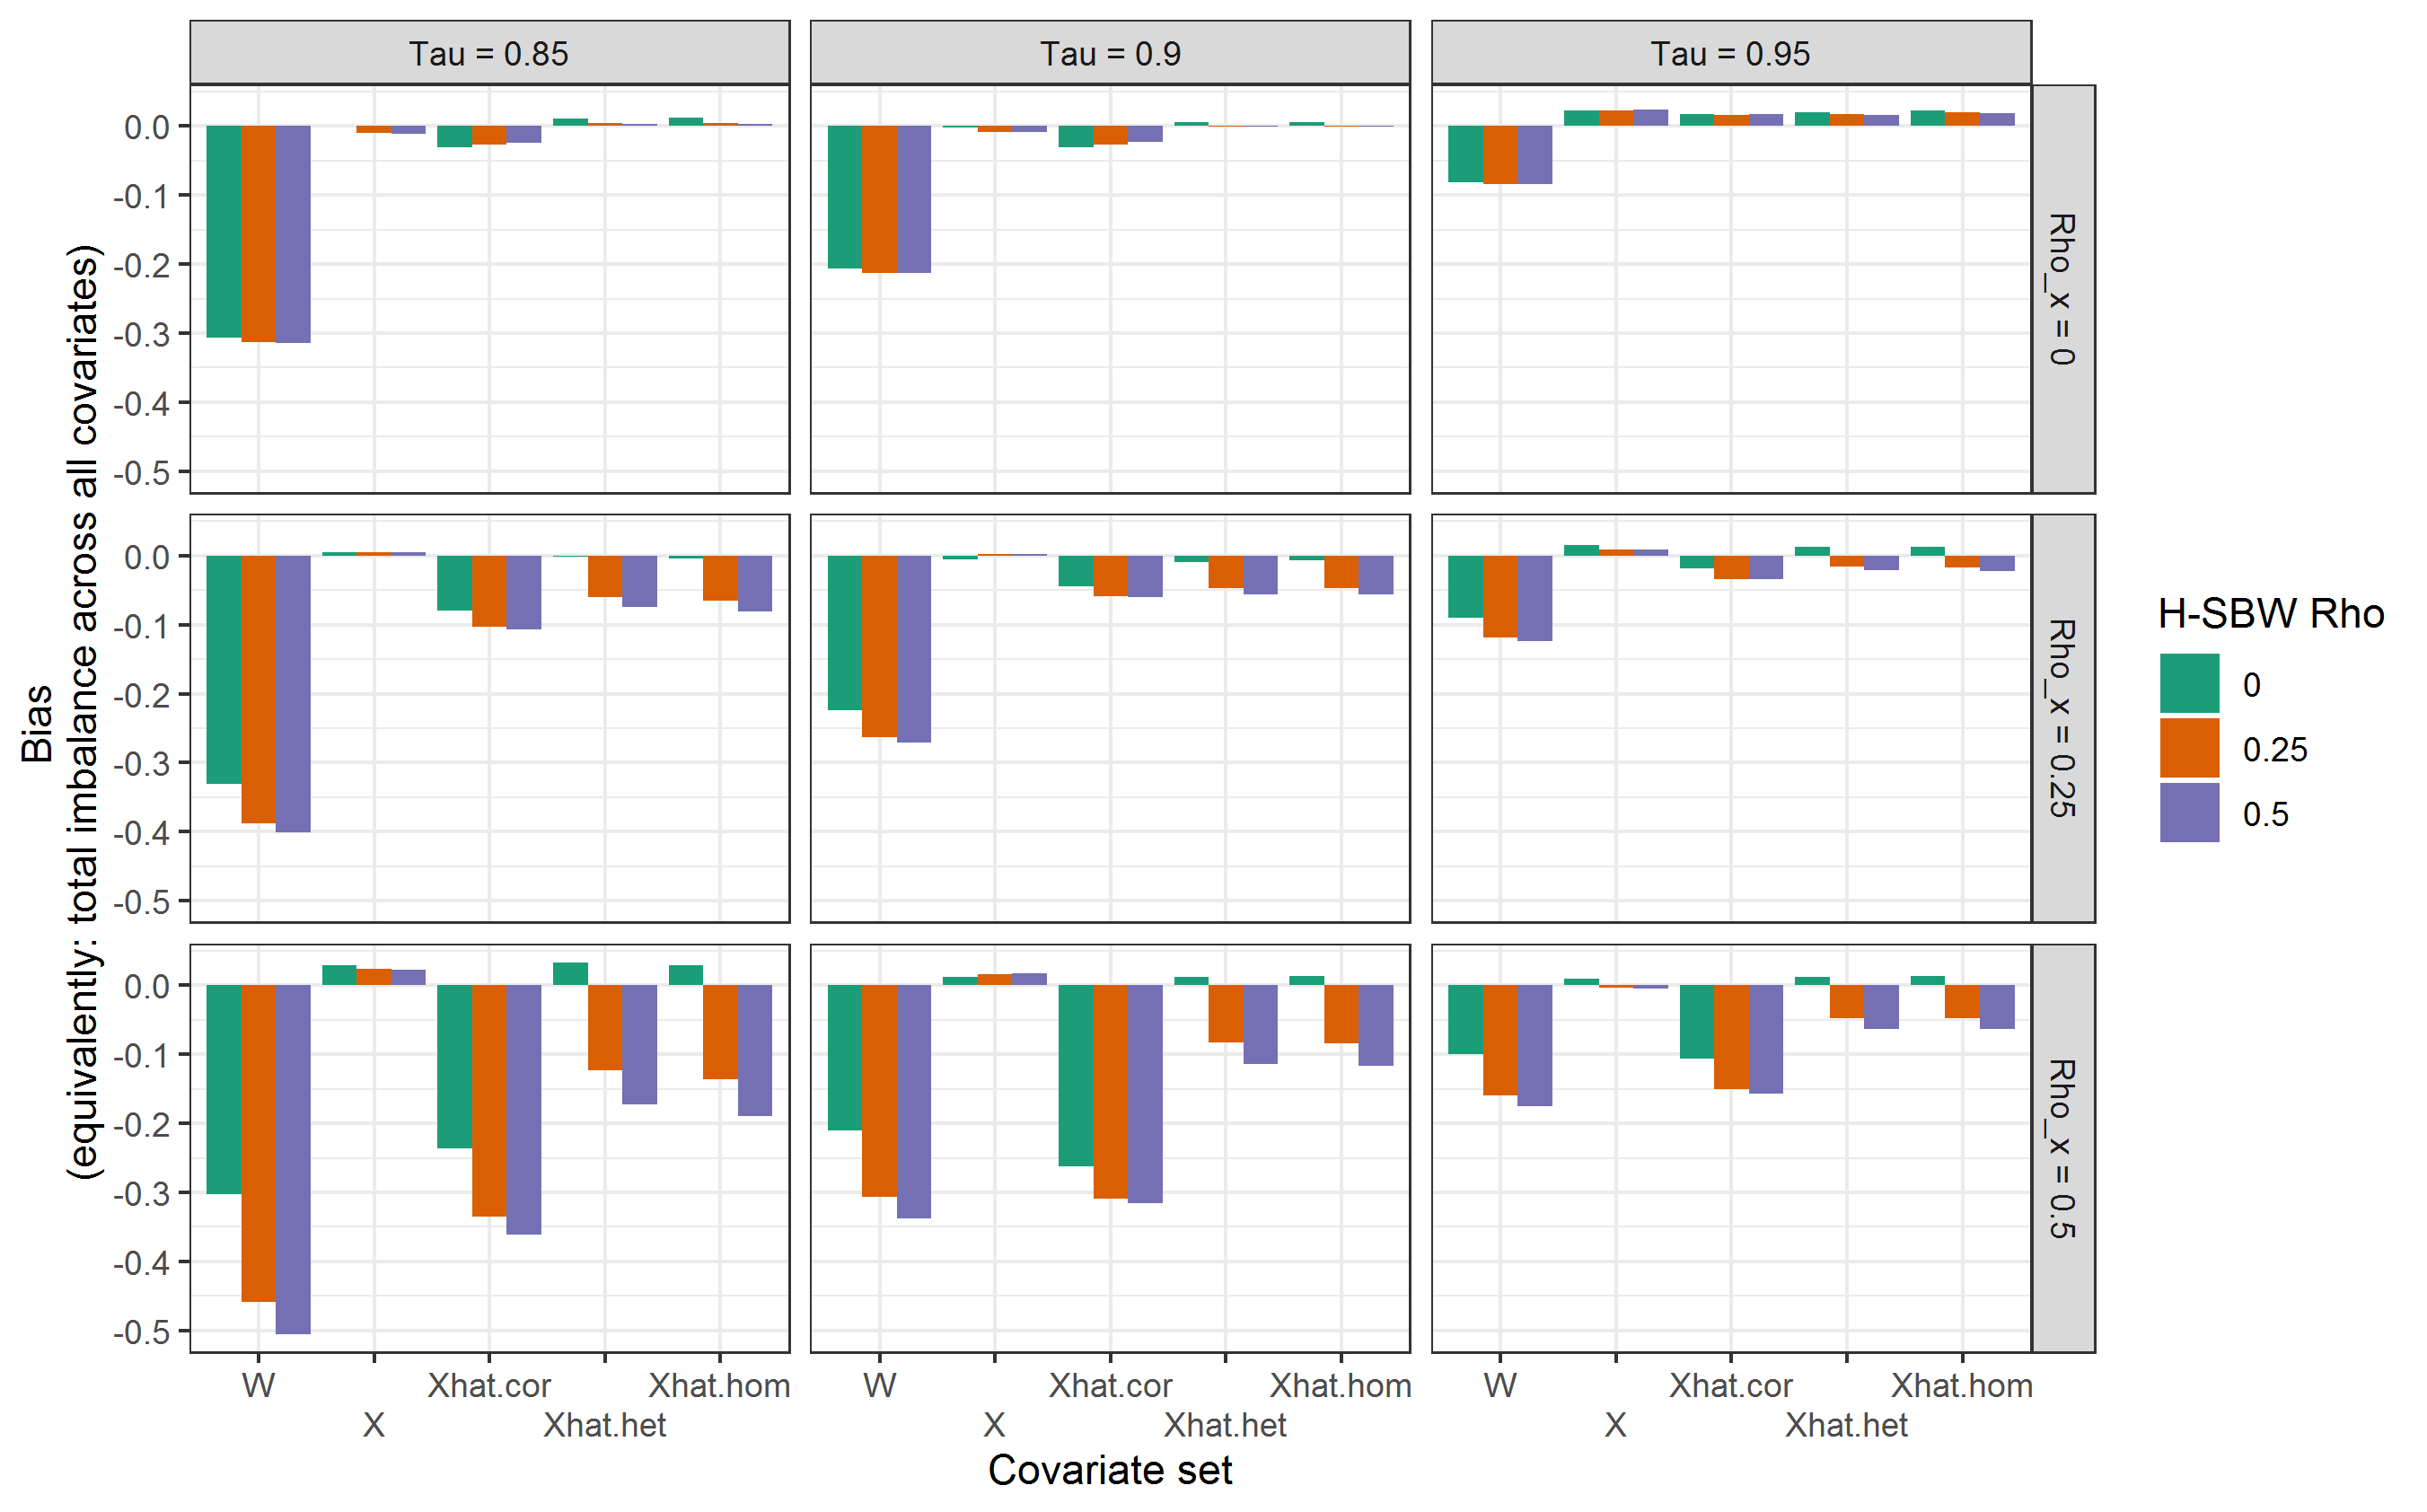
\includegraphics[scale=0.5]{01_Plots/bias-plot.png}
    \subcaption{Averaged across 500 simulations for each specification}
\end{center}
\end{figure}

All of these simulations had heterogeneous measurement. When we examine the results when the errors are homogeneous (results not displayed but available upon request), we find that the estimators that balance on $\tilde{X}^{het}$ have a small bias even when $\tau = 0$ or $\rho = 0$. Assuming this model is correct when it is not appears to have some cost. This may help explain the worse performance we found when applying the heterogeneous adjustment to our validation study in Section~\ref{sec:results}.

We next calculate the variance our estimators across all simulations and display these results in Figure~\ref{fig:simvar}. We find that we obtain a modest reduction in variance as we increase $\rho$. Even when assumed $\rho$ is far from optimal (i.e. $\rho = 0.50$), we tend to get nearly identical improvements to choosing $\rho = 0.25$ (again noting that the optimal $\rho$ in the context of measurement error is strictly less than this value). When we consider a wider range of parameterizations of $(\rho, \rho^\star)$ in a context without measurement error (see Section~\ref{appssec:simstudyresults2}) we find similar results.

We also see that balancing on $\tilde{X}^{cor}$ can lead to a much more variable estimate, particularly when the covariates have larger within-state correlations. Only in the setting with uncorrelated covariates and little measurement error does the variability induced by this adjustment not appear to have a cost.

\begin{figure}[H]
\begin{center}
    \caption{Simulation study: estimator variance}\label{fig:simvar}
    \label{fig:loveplotc1}
    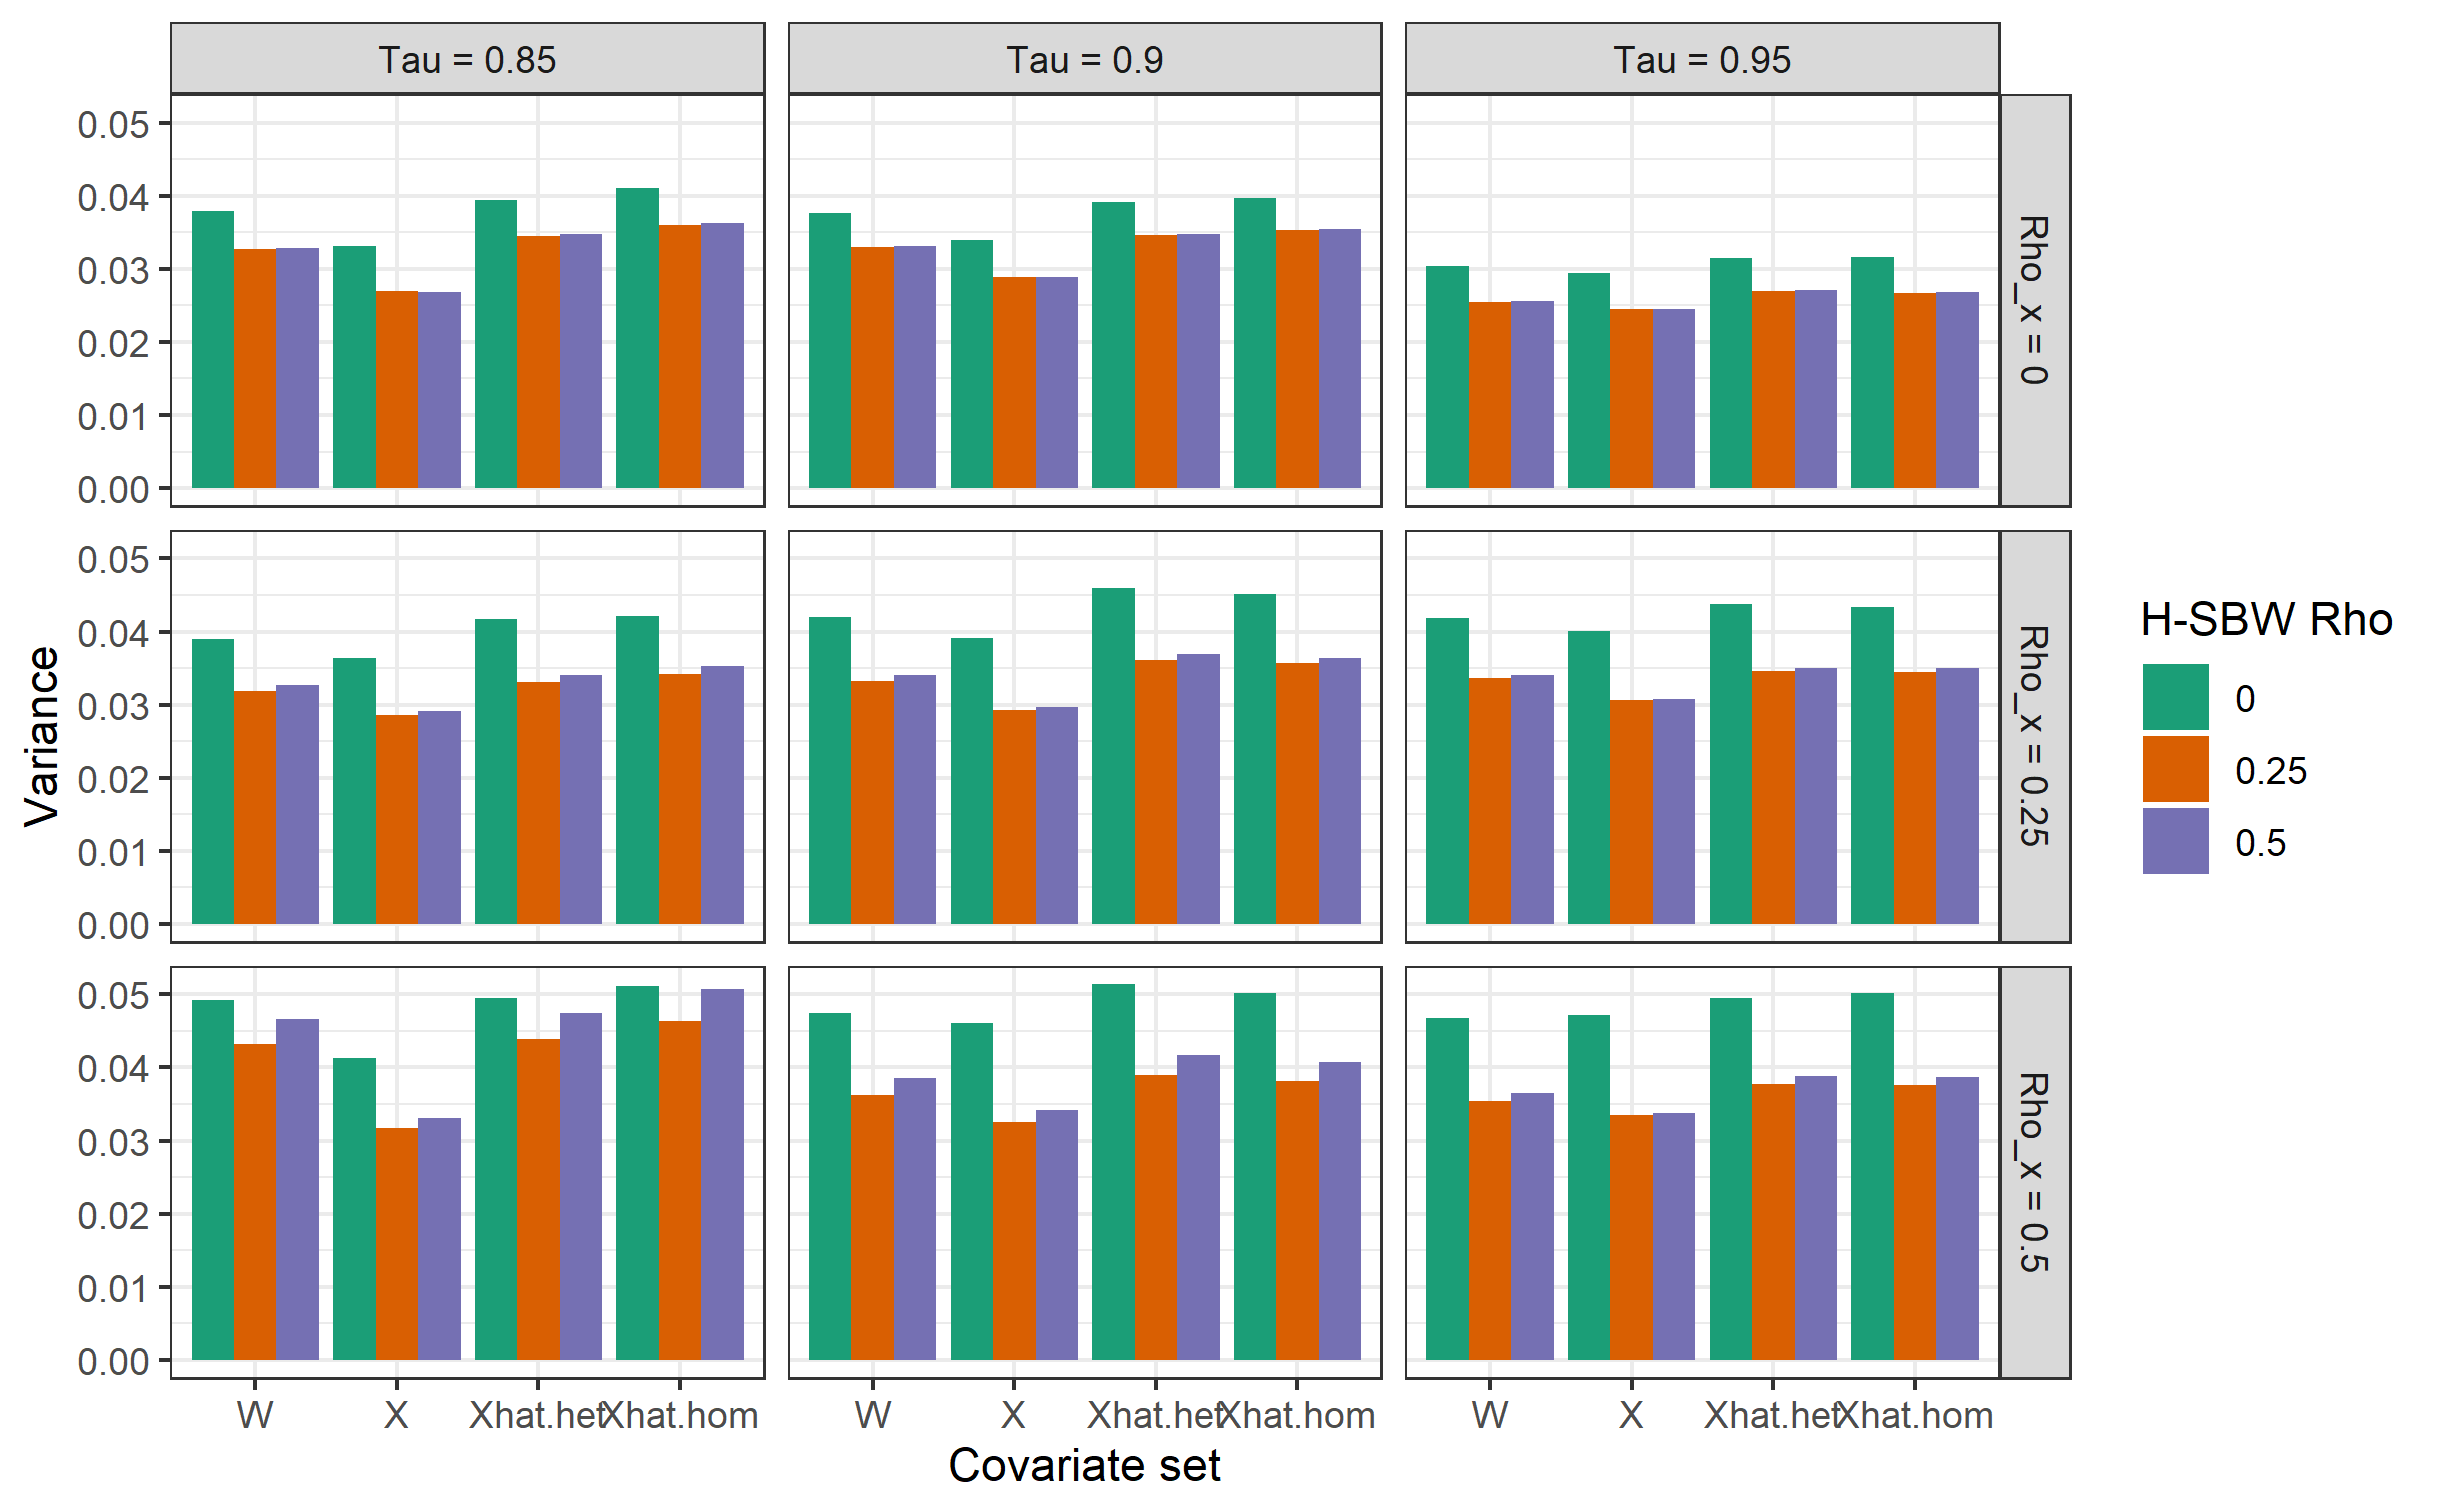
\includegraphics[scale=0.5]{01_Plots/var-plot.png}
    \subcaption{Averaged across 500 simulations for each specification}
\end{center}
\end{figure}

Figure~\ref{fig:simmse} displays the MSE of these estimators. We observe that the estimators generated on $\hat{X}^{cor}$ have larger MSE, largely driven by the increase in variability we saw previously. Despite the increase in bias for H-SBW with $\hat{X}^{hom}$ or $\hat{X}^{het}$, we may still find a modest MSE reduction when using H-SBW relative to SBW. This appears more likely as the magnitude of the measurement error measurement error decreases and/or the within-state correlation decreases (i.e. moving towards the top-right of the plot). Of course, more generally whether an MSE improvement is possible also depends on $\rho^\star$: if we were to set $\rho^\star = 0$, we would expect the MSE of these estimators to increase for all estimators as $\rho$ increases, even when we observe $X$ (see also Section~\ref{appssec:simstudyresults2}). The results are similar when considering homoskedastic measurement errors, though the space where we see MSE improvements for H-SBW relative to SBW on the uncorrelated adjustments appears to increase slightly (results available on request). 

\begin{figure}[H]
\begin{center}
    \caption{Simulation study: estimator mean-square-error}\label{fig:simmse}
    \label{fig:loveplotc1}
    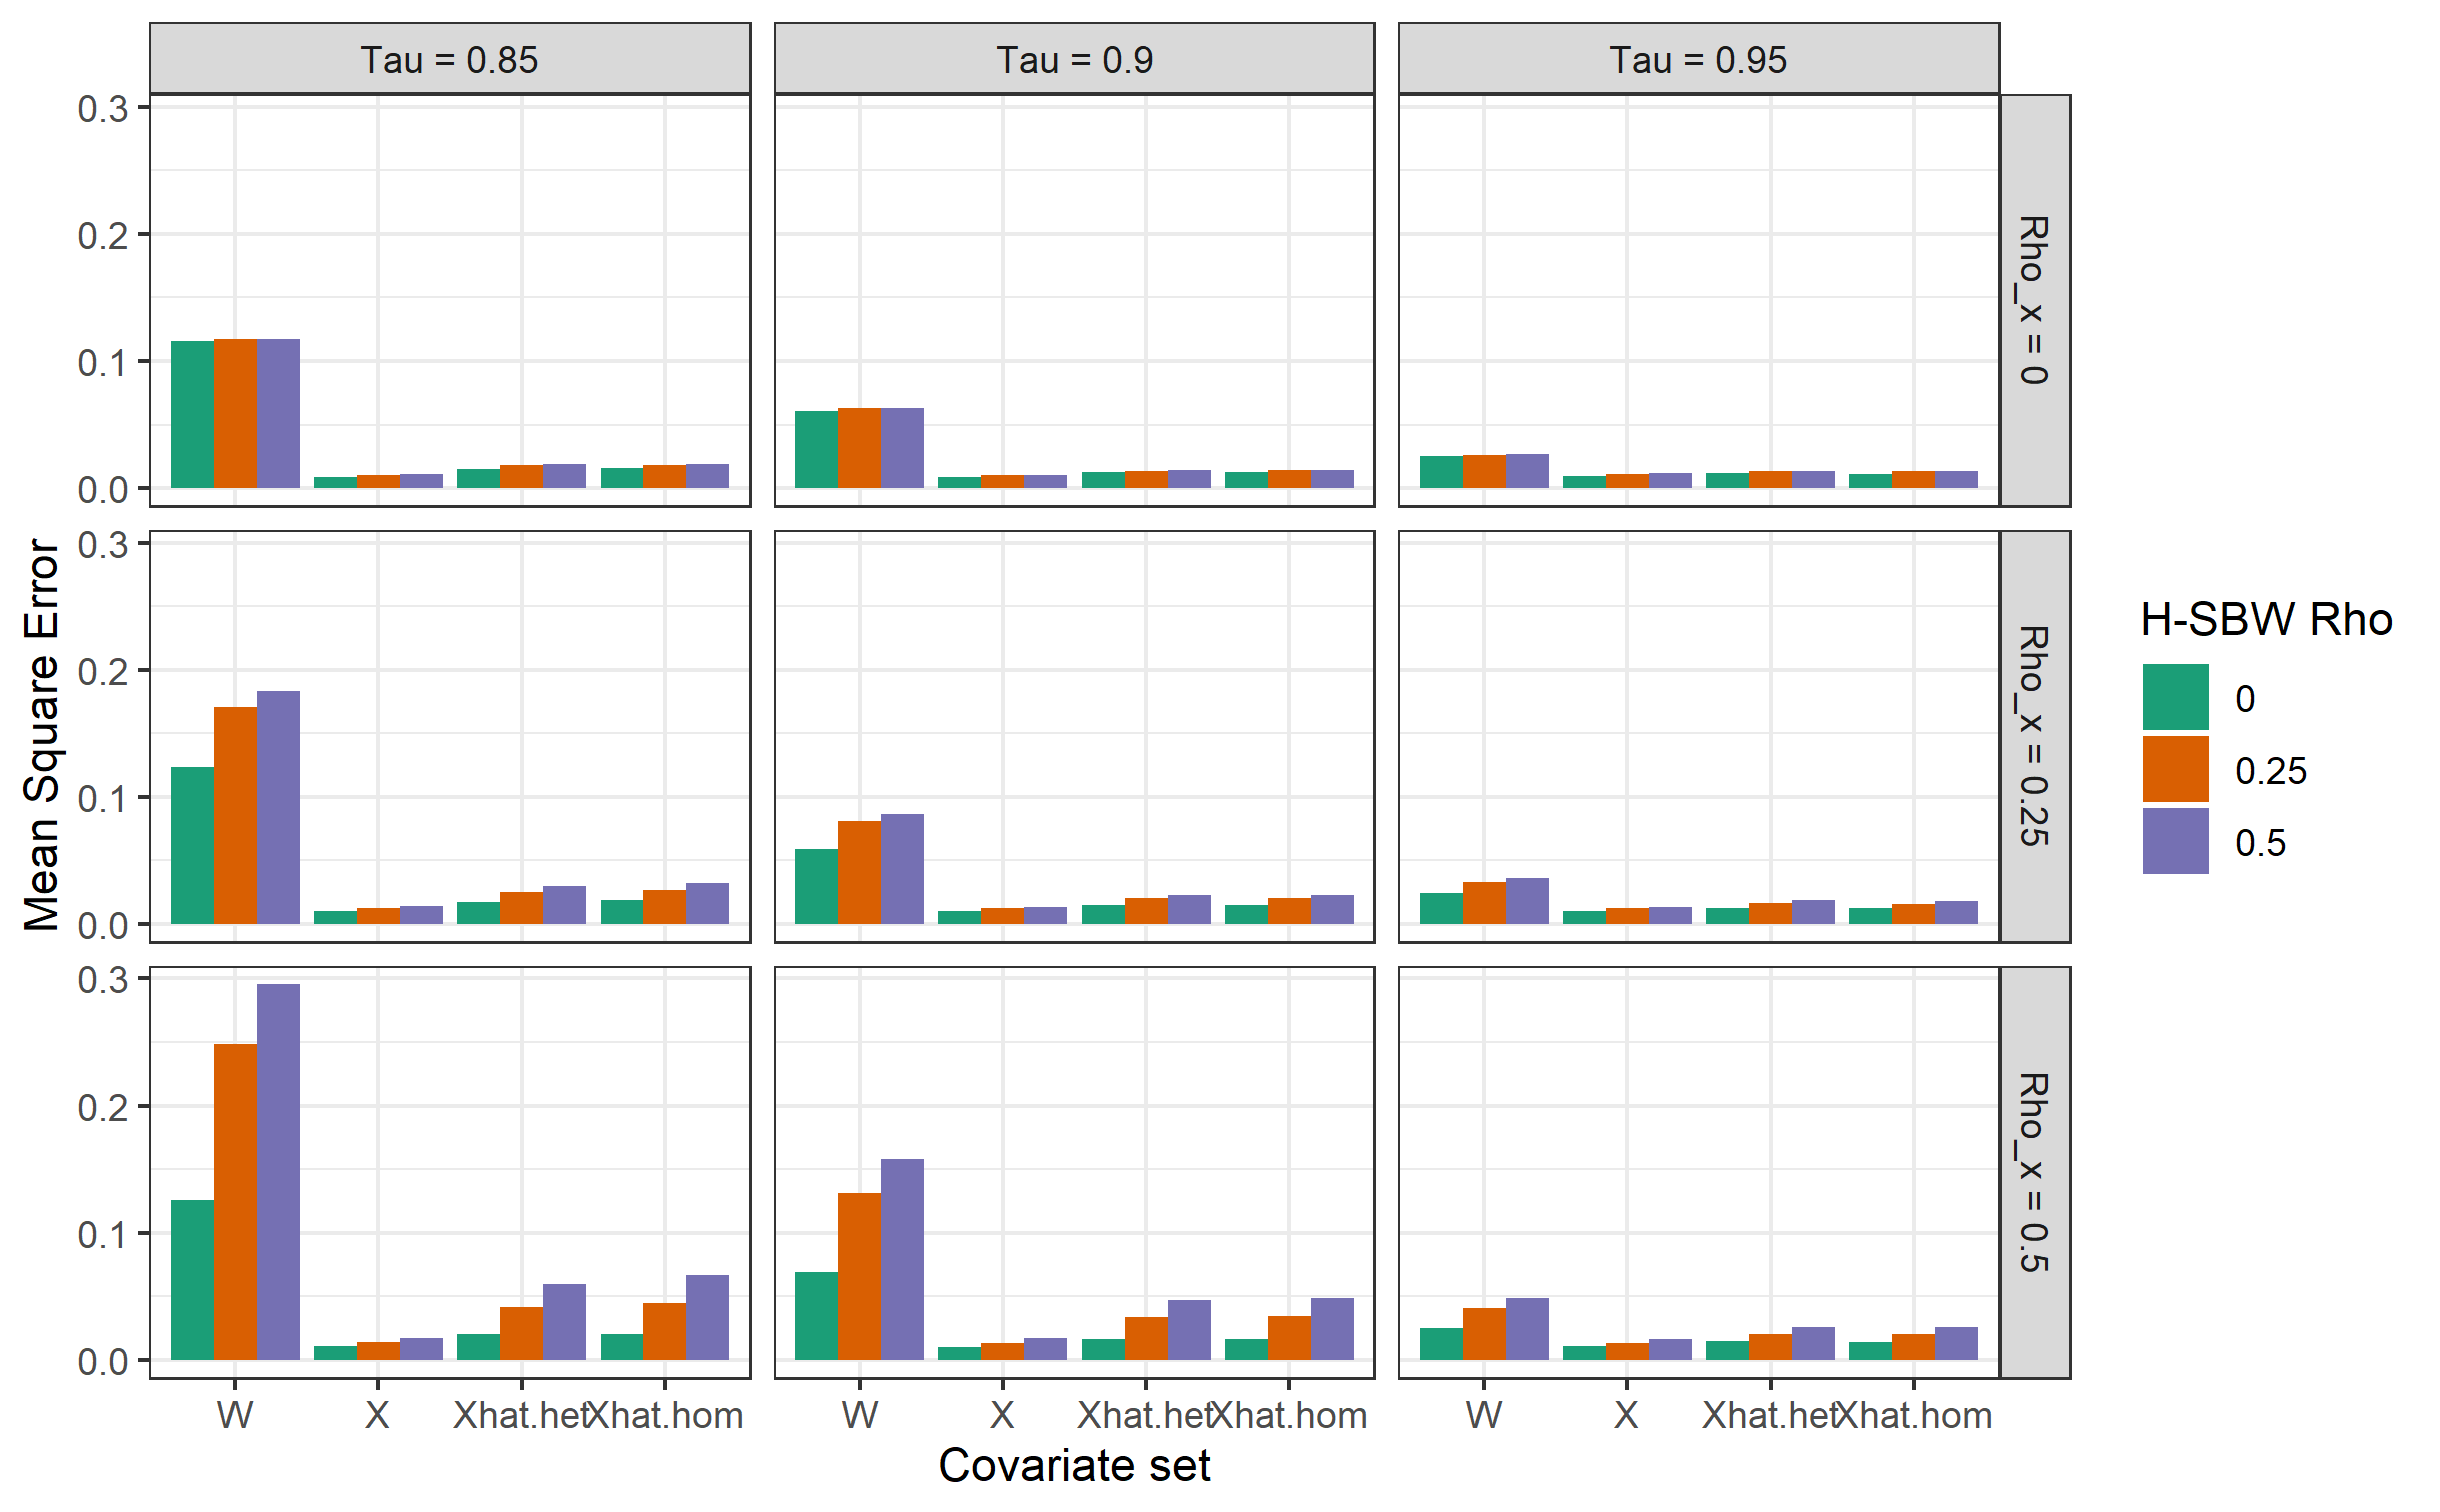
\includegraphics[scale=0.5]{01_Plots/mse-plot.png}
    \subcaption{Averaged across 500 simulations for each specification}
\end{center}
\end{figure}

We next evaluate the performance of the leave-one-state-out jackknife procedure and evaluate confidence interval coverage (for 95\% confidence intervals) and length, and display these results in Figures~\ref{fig:simcoverage1} and ~\ref{fig:simcoverage2}. 

We first discuss Figure~\ref{fig:simcoverage1}. When $\rho = 0$ we find that we obtain approximately nominal coverage rates across all specifications that use $X$ or some version of $\hat{X}$. However, we fail to get even close to nominal coverage rates when balancing on $W$, even when $\tau$ is quite high. This suggests that even when the amount of measurement error is small, so that the bias is small, our variance estimates may still not have appropriate coverage.

The performance of our variance estimates appears to deteriorate as we increase $\rho_x$, even when balancing on the true covariates. We also see that our coverage rates worsen for $\hat{X}^{het}$ and $\hat{X}^{hom}$ in the settings where we found the highest bias. On the other hand, we find that our coverage rates are often quite conservative for estimators generated on $\hat{X}$, particularly those using $\hat{X}^{cor}$. By contrast the coverage rates appear to be slightly less than desired for estimators using $X$; we investigate and discuss this further in Section~\ref{appssec:simstudyresults2}. 

\begin{figure}[H]
\begin{center}
    \caption{Simulation study: jackknife coverage rates}\label{fig:simcoverage1}
    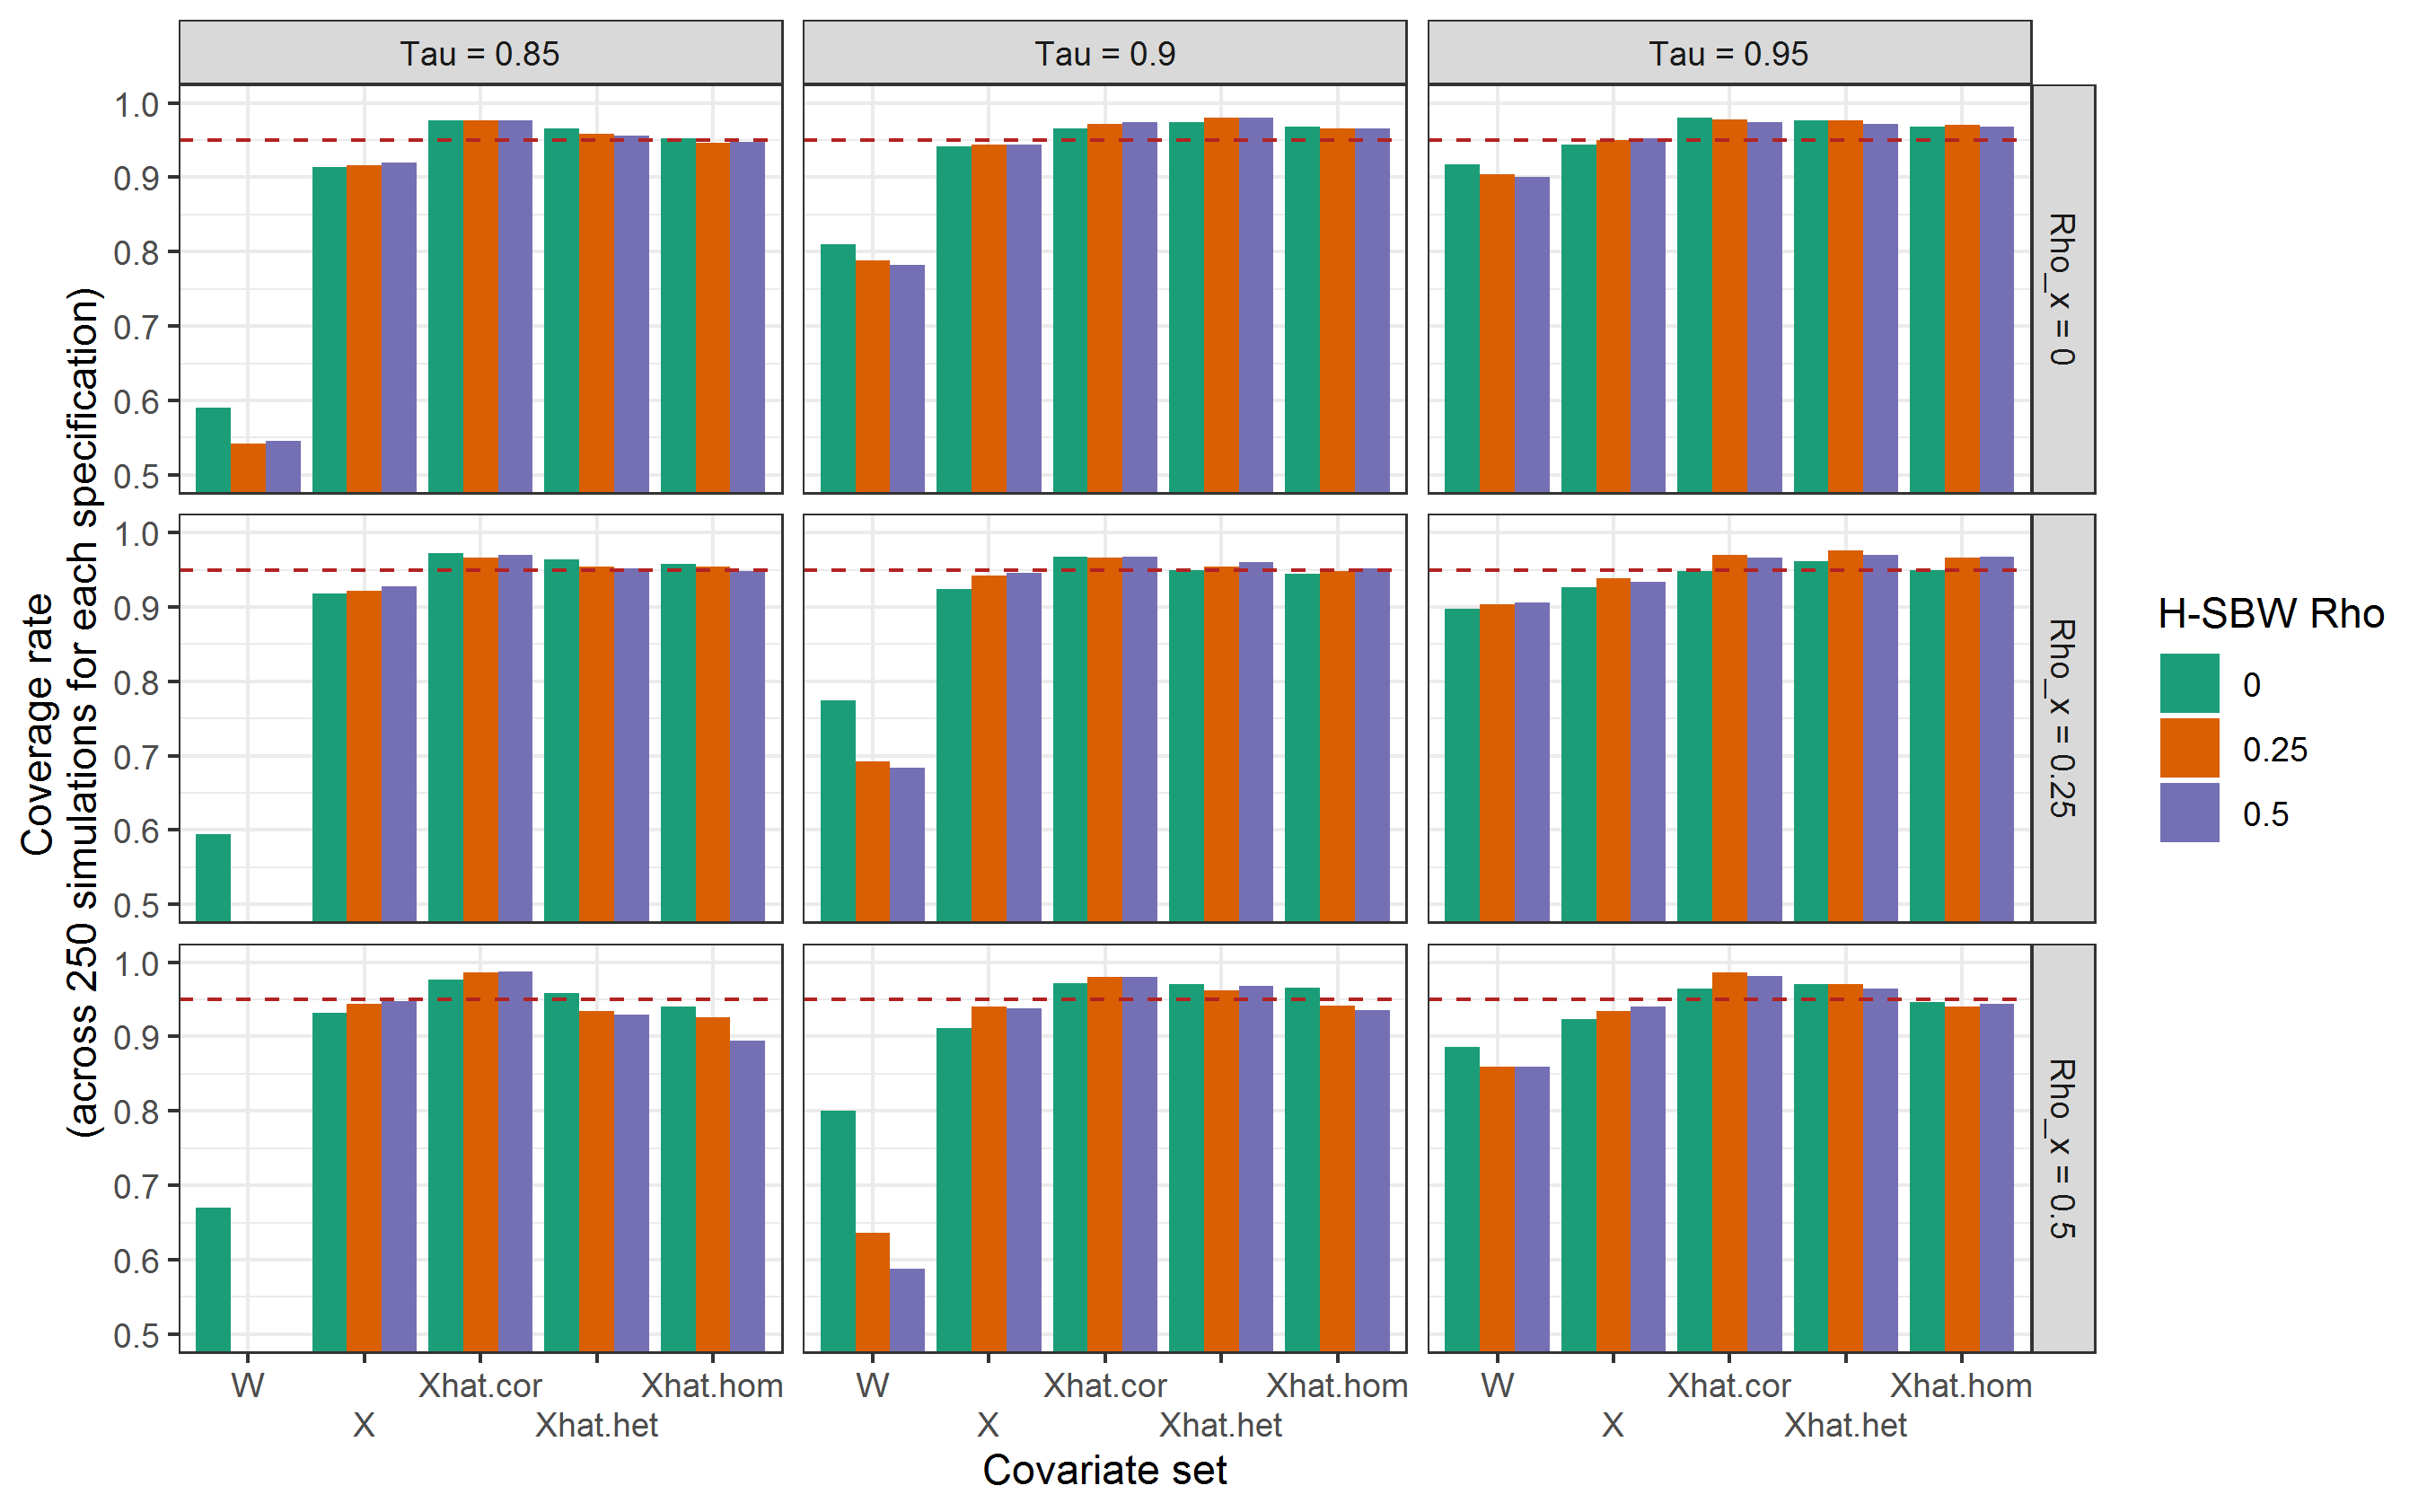
\includegraphics[scale=0.5]{01_Plots/coverage-plot-1.png}
    \subcaption{Averaged across 500 simulations for each specification}
\end{center}
\end{figure}

Figure~\ref{fig:ciwidth} compares the mean confidence interval lengths using the leave-one-state-out jackknife. We see the H-SBW estimator is associated with slightly more precise estimates, reflecting that the estimators have decreased variability under our assumed correlation structures. We again see that even when we choose $\rho$ quite sub-optimally ($\rho = 0.5$) we obtain more precise inferences than when $\rho = 0$. This again suggests benefits to using H-SBW even when our estimate of $\rho$ is a guess. As the previous results would suggest, we also find that the confidence intervals using $\hat{X}^{cor}$ are quite large. The results are similar when considering homoskedastic measurement errors. 

\begin{figure}[H]\label{fig:ciwidth}
\begin{center}
    \caption{Confidence interval length}\label{fig:simcoverage2}
    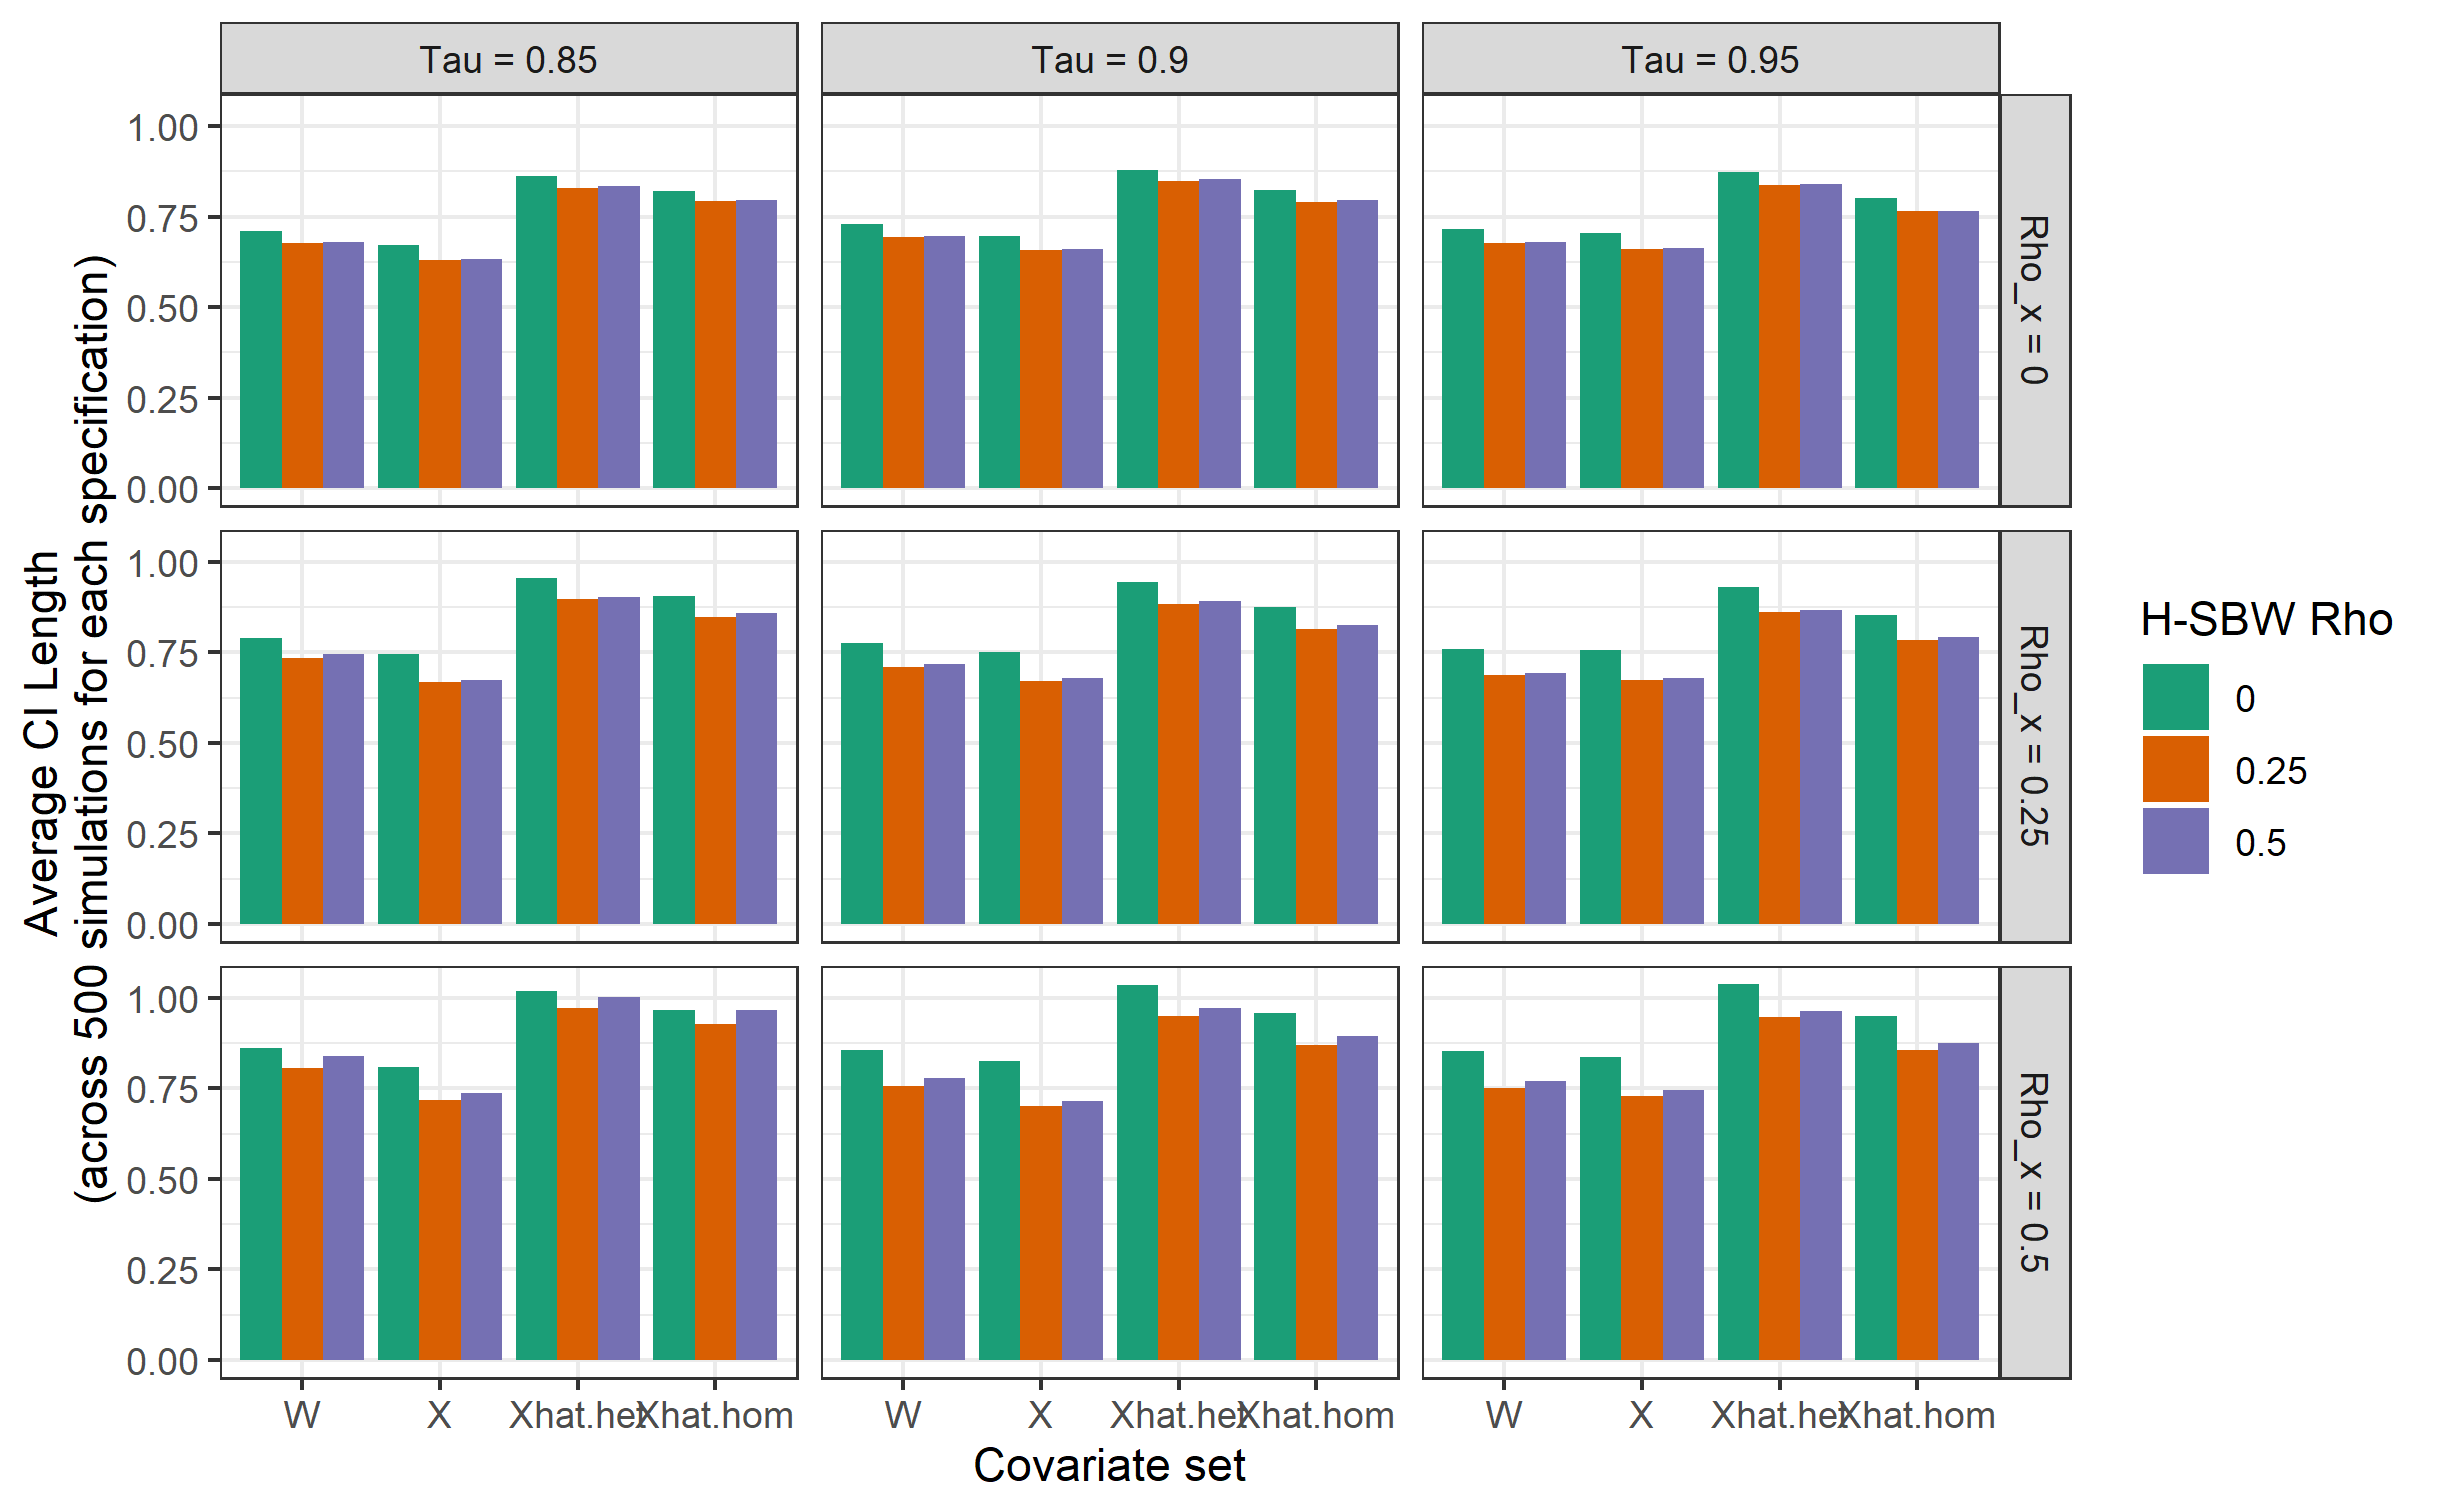
\includegraphics[scale=0.5]{01_Plots/ci-length-plot.png}
    \subcaption{Averaged across 500 simulations for each specification}
\end{center}
\end{figure}

We emphasize three takeaways from this simulation study. First, setting $\rho > 0$ can increase the bias of our estimates in the context of measurement error; however, the bias is generally small relative to the bias of balancing on the noisy covariate measurements $W$, and MSE improvements using H-SBW are still possible relative to SBW despite the bias. Second, accounting for the correlation in the data when using H-SBW and the data are measured with error may not be worth the cost in variance given a small sample of states, despite the improved theoretic properties. This simulation study assumes throughout that we know the true data generating model for the outcome, and that are data are gaussian. Finally, we find no evidence that the ``heterogeneous adjustment'' improves our estimates along any dimension, even in an ideal setting. Moreover this adjustment may even induce bias when the model is incorrect. This finding may in part reflect the distribution of sample sizes we generated, which we took to be uniform; perhaps with a different distribution these results would differ. Overall this study complements our validation study in Section~\ref{sec:results}, which has more direct bearing on understanding how these estimators might perform in our application.

\subsection{Additional results: H-SBW without measurement error}\label{appssec:simstudyresults2}

We consider additional simulations for the setting where $X$ is known and the outcome model follows homoskedastic but possibly correlated errors. For these results we only vary $\rho^\star \in \{0, 0.25, 0.5, 0.75, 0.99\}$, and fix $\rho_x = 0.25$ throughout. 

Figure~\ref{fig:hsbwvarx} displays the empirical variance of the H-SBW estimators averaged over 1000 simulations. Each panel reflects different values of $\rho^\star$, while the x-axis throughout displays the assumed value of $\rho$ in the H-SBW objective. The red bars indicate when $\rho$ is optimally selected -- $\rho = \rho^\star$. We see that this selection corresponds with the lowest variance estimator, we would expect. Consistent with our previous results, we find that when $\rho^\star > 0$, we find that any assumed $\rho$ improves the variance of the resulting estimator relative to SBW. Of course, this requires in general that our assumed correlation structure of the error terms is correct.

\begin{figure}[H]
\begin{center}
    \caption{Variance of H-SBW estimator for known covariates}\label{fig:hsbwvarx}
    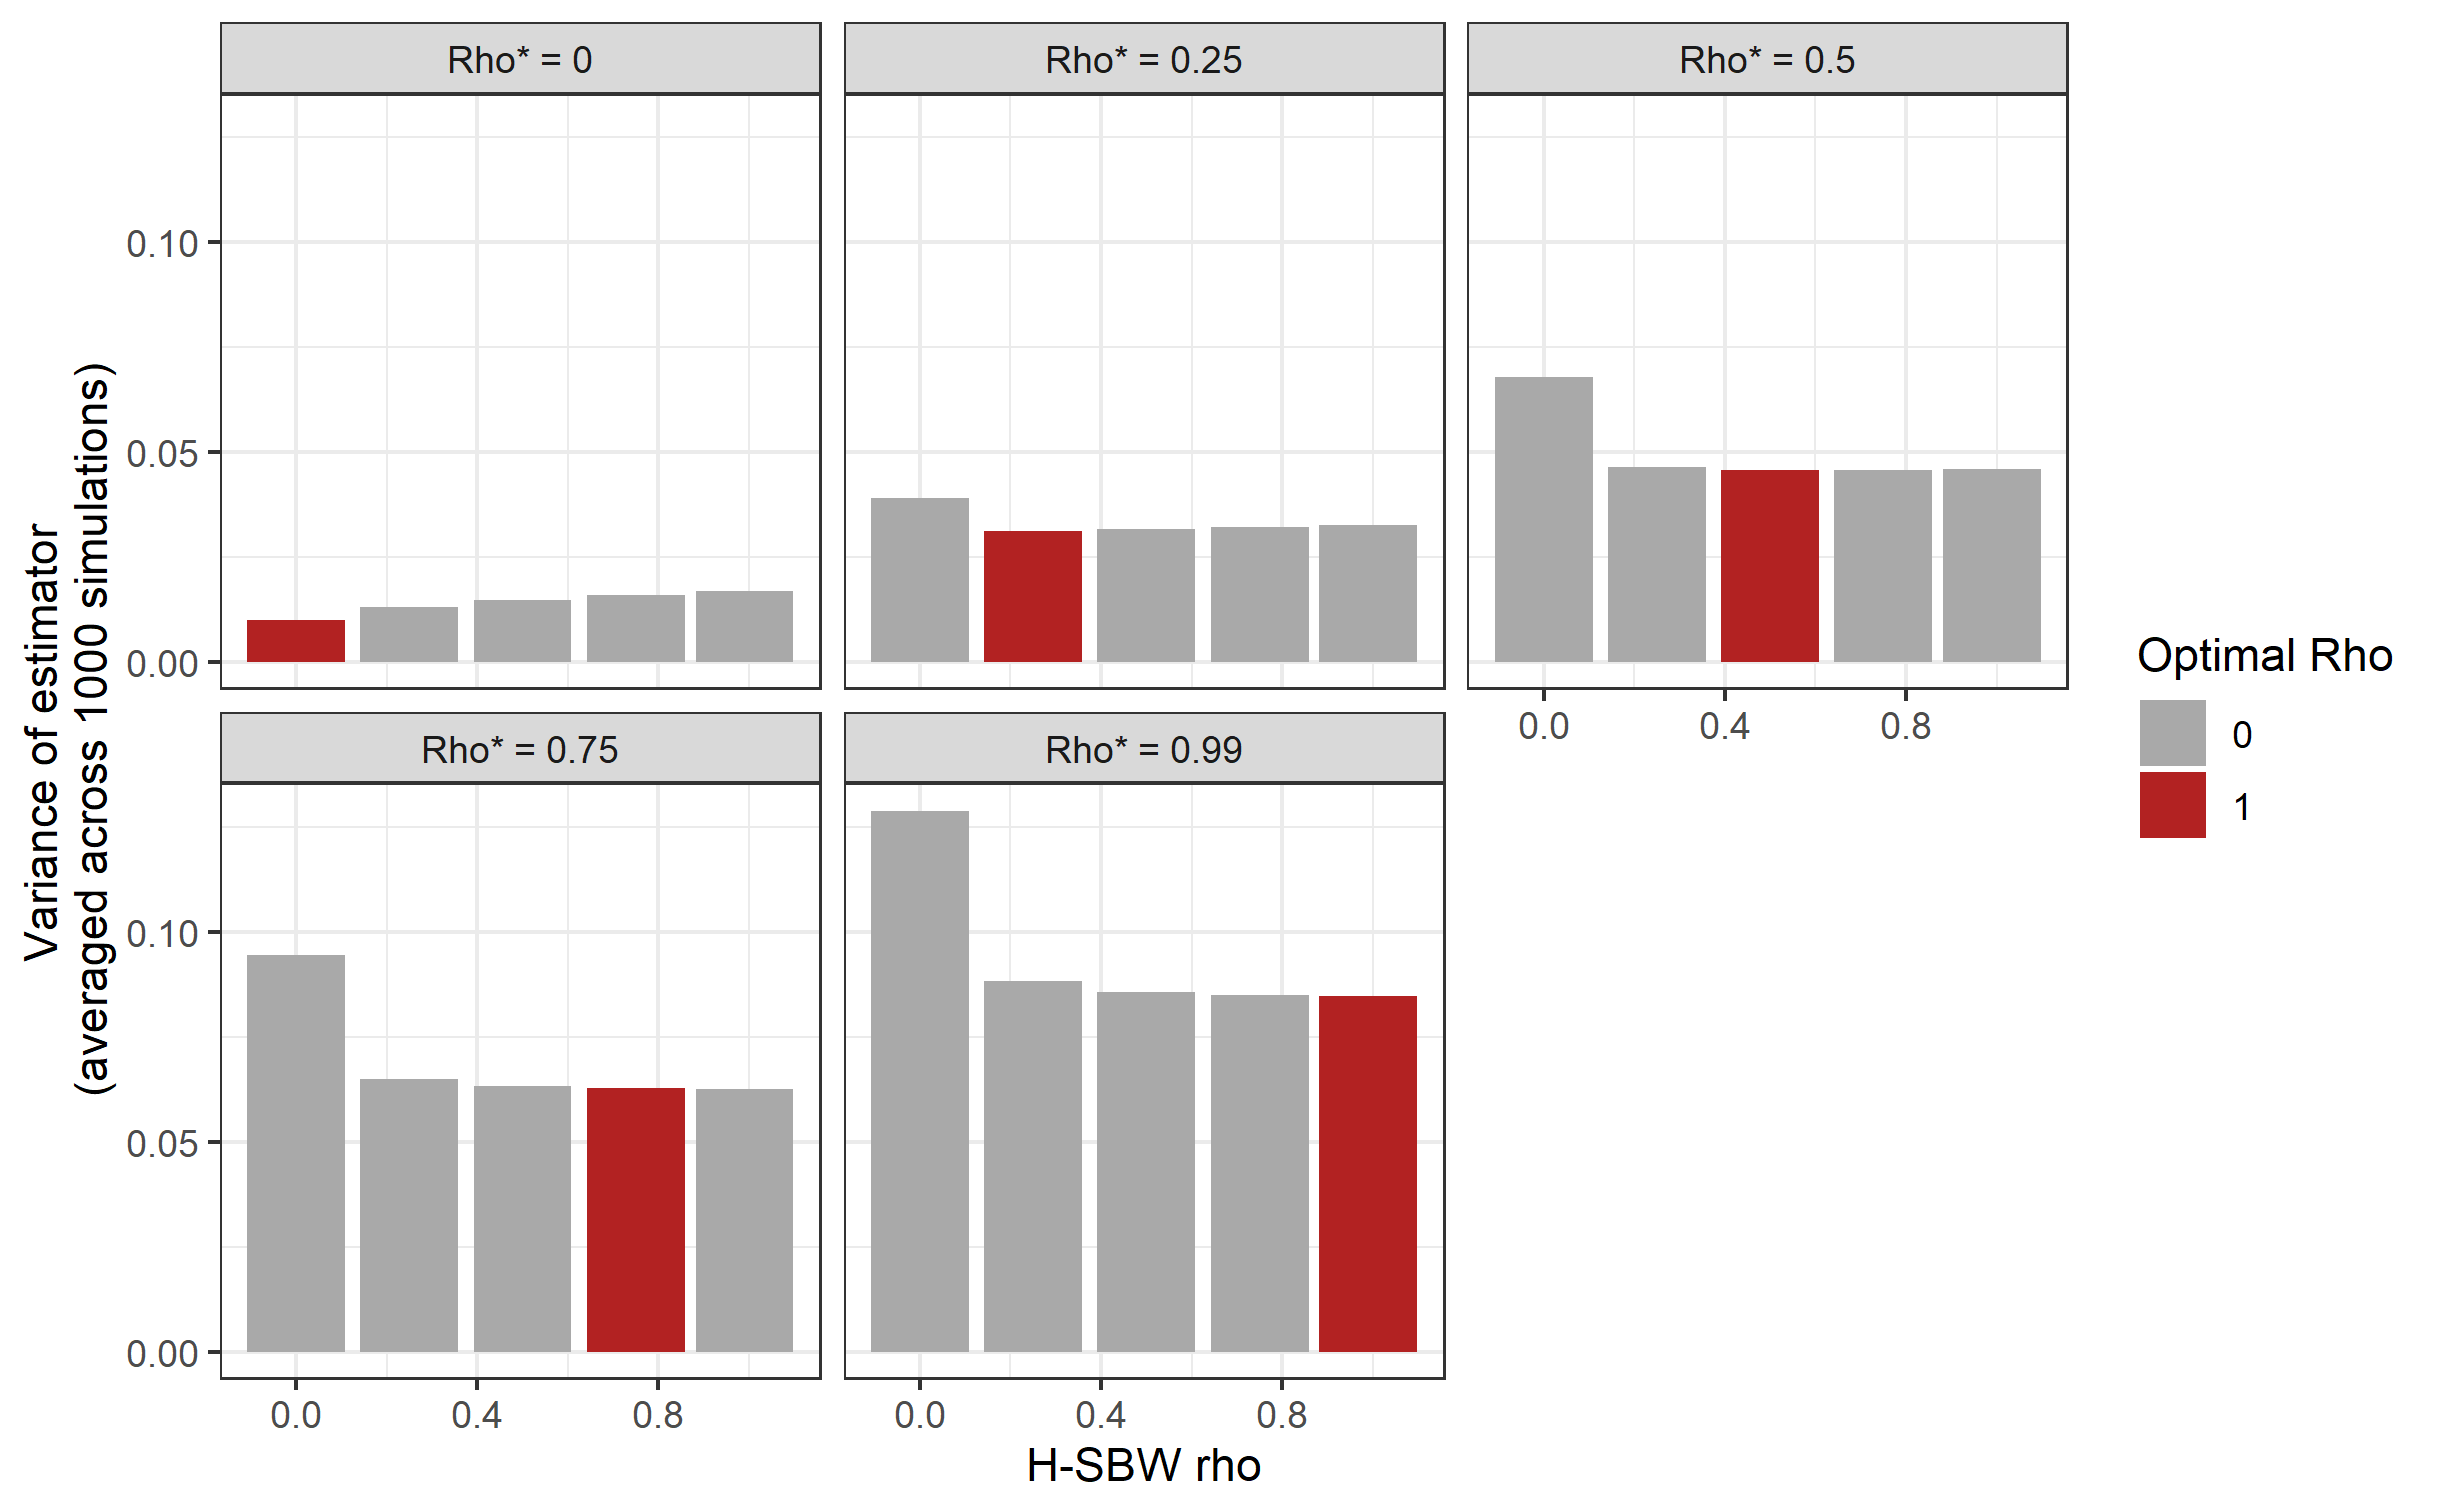
\includegraphics[scale=0.5]{01_Plots/variance-x-plot.png}
    \subcaption{Averaged across 1000 simulations for each specification}
\end{center}
\end{figure}

We conclude by examining the confidence interval coverage for the leave-one-state-out-jackknife. Figure~\ref{fig:hsbwcoveragex} displays the results. Consistent with our previous findings, we see that we generally obtain slightly less than nominal coverage rates, particularly when $\rho^\star$ is small. We speculate that this may be a function of the jackknife being an approximation to the bootstrap, which itself is only an asymptotically unbiased estimate of the variance. Given our sample of $m_1 = 25$, this slight under-coverage is not entirely surprising. On the other hand, this does contrast with our finding that this procedure in general is conservative in the presence of measurement error. 

We conclude by observing that coverage improves when setting $\rho > 0$, even when $\rho^\star = 0$. We speculate that by more evenly dispersing the weights across states, H-SBW may be increasing the effective sample size of states, improving the asymptotic approximation of the jackknife. This again illustrates a possible value of using this procedure. Analyzing the theoretic properties of these variances estimators to better understand these results in this setting would be useful future work; however, this is beyond the scope of the present study.

\begin{figure}[H]
\begin{center}
    \caption{H-SBW coverage for known covariates}\label{fig:hsbwcoveragex}
    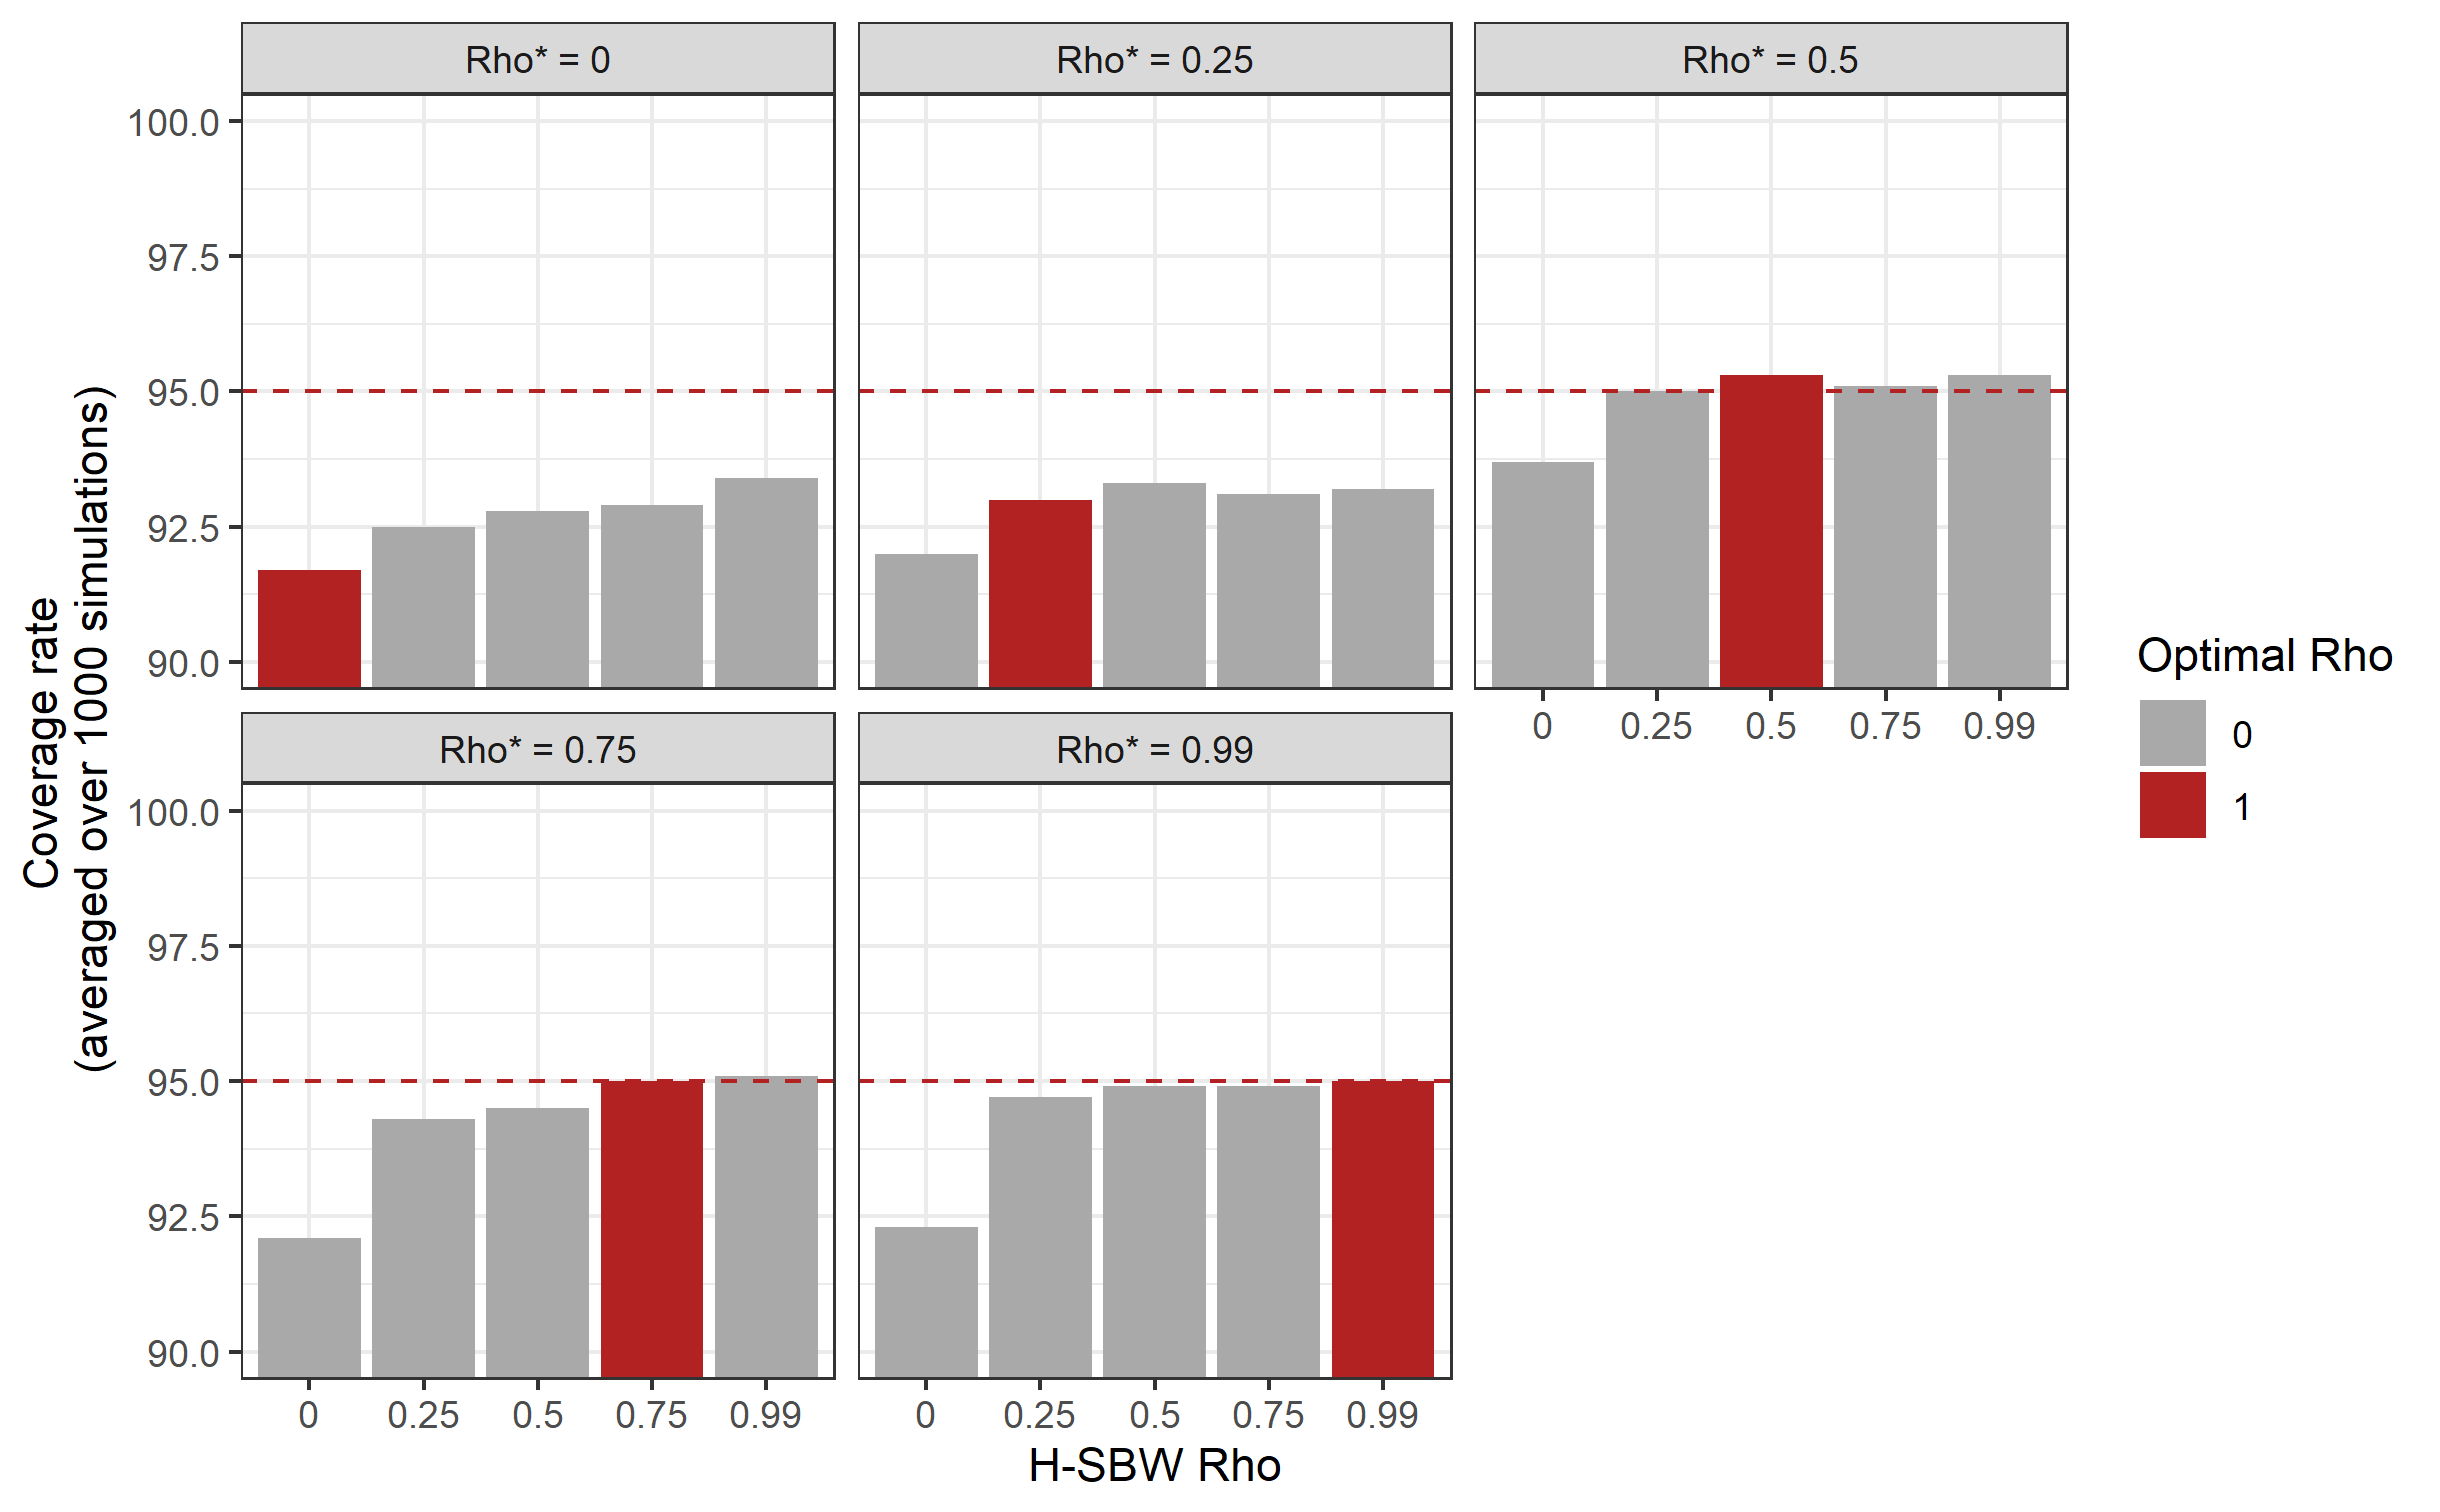
\includegraphics[scale=0.5]{01_Plots/coverage-x-plot.png}
    \subcaption{Averaged across 1000 simulations for each specification}
\end{center}
\end{figure}